\documentclass[12pt]{article}

\usepackage{amsmath}
\usepackage{array}
\usepackage{caption}
\usepackage[margin=1in]{geometry}
\usepackage{graphicx}
\usepackage[colorlinks=true, allcolors=blue]{hyperref}
\usepackage[utf8]{inputenc}
\usepackage{multirow}
\usepackage[section]{placeins}

\graphicspath{{./figures/}}

\title{ECE 271: Chapter 2 Reading Report}
\author{Phi Luu}
\date{\today}

\begin{document}

\maketitle

%%%%%%%%%%%%%%%%%%%%%%%%%%%%%%%%%%%%%%%%%%%%%%%%%%%%%%%%%%%%%%%%%%%%%%%%%%%%%%%%
% Chapter Outline
%%%%%%%%%%%%%%%%%%%%%%%%%%%%%%%%%%%%%%%%%%%%%%%%%%%%%%%%%%%%%%%%%%%%%%%%%%%%%%%%
\section{Chapter Outline}

This chapter covers the basics of combinational logic design and heavily focuses on the functional and timing relationships between inputs and outputs of a circuit. In this chapter, the authors use boolean and boolean algebra to explain multilevel combinational logic and apply these concepts to make hardware reduction for more complex circuits. Another focus of this chapter is showing how to use Karnaugh maps (or K-maps) to minimize logic in a more graphical and intuitive way. Each of the mentioned topics will be discussed further throughout the following sections.

\begin{enumerate}
    %%%%%%%%%%%%%%%%%%%%%%%%%%%%%%%%%%%%%%%%
    % Introduction
    %%%%%%%%%%%%%%%%%%%%%%%%%%%%%%%%%%%%%%%%
    \item \textbf{Introduction}

    A \textit{circuit} is a network that processes discrete-valued variables. A circuit needs to have the following:

    \begin{itemize}
        \item one or more discrete-valued \textit{input} terminals
        \item one or more discrete-valued \textit{output} terminals
        \item a \textit{functional specification} describing the relationship between the inputs and the outputs
        \item a \textit{timing specification} describing the delay between the changes in the inputs and the responses of the outputs
    \end{itemize}

    A circuit can be viewed as a black box similar to the figure below:

    \begin{figure}[h]
        \centering
        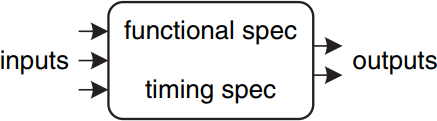
\includegraphics[width=0.5\textwidth]{circuit.png}
        \caption{A circuit as a black box with inputs, outputs, and specifications}
        \label{Figure 2.1}
    \end{figure}

    \newpage

    A circuit has two components:

    \begin{itemize}
        \item \textit{Elements}: An element is itself a circuit with inputs, outputs, and specifications.
        \item \textit{Nodes}: A node is a wire whose voltage is discrete-valued. Nodes are further classified into three types:
        \begin{itemize}
            \item \textit{Inputs} receive values from the external world.
            \item \textit{Outputs} deliver values to the external world.
            \item \textit{Internals} are wires that are neither inputs nor outputs.
        \end{itemize}
    \end{itemize}

    Digital circuits are classified as \textit{combinational} or \textit{sequential}. A combinational circuit is memoryless; its outputs depend only on the current values of the inputs. Recall the logic gates from chapter 1, they are examples of a combinational circuit. A sequential circuit, on the other hand, has memory; its outputs depend on both the current values of the inputs and the previous values of the inputs. This chapter focuses on combinational circuits, and chapter 3 will cover sequential circuits.

    A circuit is combinational if it consists of interconnected circuit elements such that

    \begin{itemize}
        \item Every circuit element is combinational.
        \item Every node is either an input to the circuit or connected to \textit{exactly one} output terminal of an element.
        \item There are no cyclic paths.
    \end{itemize}

    The functional specification of a circuit is often expressed as a truth table or a Boolean equation which will be discussed in the next subsection.

    %%%%%%%%%%%%%%%%%%%%%%%%%%%%%%%%%%%%%%%%
    % Boolean Equations
    %%%%%%%%%%%%%%%%%%%%%%%%%%%%%%%%%%%%%%%%
    \item \textbf{Boolean Equations}

    Boolean equations deal with variables that are either TRUE or FALSE. Therefore, they are perfect for describing digital logic. The table below shows the terminologies, notations, and truth tables of some commonly used Boolean equations.

    \begin{center}
        \begin{tabular}{ | c | >{\centering\arraybackslash}p{6em} | >{\centering\arraybackslash}p{2em} | >{\centering\arraybackslash}p{2em} | >{\centering\arraybackslash}p{4em} | }
        \hline
        \textbf{Terminology}                              & \textbf{Notation}          & \multicolumn{3}{c|}{\textbf{Truth Table}}                               \\ \hline \rule{0cm}{1em}
        \multirow{3}{*}{Complement of $A$}                & \multirow{3}{*}{$\bar{A}$} & \multicolumn{2}{c|}{$\mathbf{A}$} & $\mathbf{\bar{A}}$                  \\ \cline{3-5} \rule{0cm}{1em}
                                                          &                            & \multicolumn{2}{c|}{0}            & 1                                   \\ \cline{3-5} \rule{0cm}{1em}
                                                          &                            & \multicolumn{2}{c|}{1}            & 0                                   \\ \hline \rule{0cm}{1em}
        \multirow{5}{*}{Product/Implicant of $A$ and $B$} & $AB$                       & $\mathbf{A}$    & $\mathbf{B}$    & $\mathbf{AB}$                       \\ \cline{2-5} \rule{0cm}{1em}
                                                          & $A$ AND $B$                & 0               & 0               & 0                                   \\ \cline{2-5} \rule{0cm}{1em}
                                                          & \multirow{3}{*}{}          & 0               & 1               & 0                                   \\ \cline{3-5} \rule{0cm}{1em}
                                                          &                            & 1               & 0               & 0                                   \\ \cline{3-5} \rule{0cm}{1em}
                                                          &                            & 1               & 1               & 1                                   \\ \hline \rule{0cm}{1em}
        \multirow{5}{*}{Sum of $A$ and $B$}               & $A + B$                    & $\mathbf{A}$    & $\mathbf{B}$    & $\mathbf{A + B}$                    \\ \cline{2-5} \rule{0cm}{1em}
                                                          & $A$ OR $B$                 & 0               & 0               & 0                                   \\ \cline{2-5} \rule{0cm}{1em}
                                                          & \multirow{3}{*}{}          & 0               & 1               & 1                                   \\ \cline{3-5} \rule{0cm}{1em}
                                                          &                            & 1               & 0               & 1                                   \\ \cline{3-5} \rule{0cm}{1em}
                                                          &                            & 1               & 1               & 1                                   \\
        \hline
        \end{tabular}
    \end{center}

    A \textit{minterm} is a \textbf{product} involving all variables of the inputs to the function. A \textit{maxterm} is a \textbf{sum} involving all variables of the inputs to the function.

    When multiple Boolean variables take part in a Boolean equation, the \textit{order of operations} is vital to determinant the result of the equation---similarly to the order of operations in decimal-based algebra. In Boolean equations, \textbf{NOT has the highest precedence, followed by AND, and then OR}. For instance, the Boolean equation:

    \begin{equation}
        Y = \bar{A}B + BC\bar{D}
    \end{equation}

    can be interpreted as
    \begin{equation}
        Y = ((\bar{A})B) + (BC(\bar{D})) = ((\text{NOT }A) \text{ AND }B)\text{ OR }(B \text{ AND } C \text{ AND } (\text{NOT } D))
    \end{equation}


    %%%%%%%%%%%%%%%%%%%%%%%%%%%%%%%%%%%%%%%%
    % Boolean Algebra
    %%%%%%%%%%%%%%%%%%%%%%%%%%%%%%%%%%%%%%%%
    \item \textbf{Boolean Algebra}

    %%%%%%%%%%%%%%%%%%%%%%%%%%%%%%%%%%%%%%%%
    % From Logic to Gates
    %%%%%%%%%%%%%%%%%%%%%%%%%%%%%%%%%%%%%%%%
    \item \textbf{From Logic to Gates}

    %%%%%%%%%%%%%%%%%%%%%%%%%%%%%%%%%%%%%%%%
    % Multilevel Combinational Logic
    %%%%%%%%%%%%%%%%%%%%%%%%%%%%%%%%%%%%%%%%
    \item \textbf{Multilevel Combinational Logic}

    %%%%%%%%%%%%%%%%%%%%%%%%%%%%%%%%%%%%%%%%
    % X's and Z's, Oh My
    %%%%%%%%%%%%%%%%%%%%%%%%%%%%%%%%%%%%%%%%
    \item \textbf{X's and Z's, Oh My}

    %%%%%%%%%%%%%%%%%%%%%%%%%%%%%%%%%%%%%%%%
    % Karnaugh Maps
    %%%%%%%%%%%%%%%%%%%%%%%%%%%%%%%%%%%%%%%%
    \item \textbf{Karnaugh Maps}

    %%%%%%%%%%%%%%%%%%%%%%%%%%%%%%%%%%%%%%%%
    % Combinational Building Blocks
    %%%%%%%%%%%%%%%%%%%%%%%%%%%%%%%%%%%%%%%%
    \item \textbf{Combinational Building Blocks}

    %%%%%%%%%%%%%%%%%%%%%%%%%%%%%%%%%%%%%%%%
    % Timing
    %%%%%%%%%%%%%%%%%%%%%%%%%%%%%%%%%%%%%%%%
    \item \textbf{Timing}

    %%%%%%%%%%%%%%%%%%%%%%%%%%%%%%%%%%%%%%%%
    % Summary
    %%%%%%%%%%%%%%%%%%%%%%%%%%%%%%%%%%%%%%%%
    \item \textbf{Summary}

\end{enumerate}

%%%%%%%%%%%%%%%%%%%%%%%%%%%%%%%%%%%%%%%%%%%%%%%%%%%%%%%%%%%%%%%%%%%%%%%%%%%%%%%%
% Grey Box Exploration
%%%%%%%%%%%%%%%%%%%%%%%%%%%%%%%%%%%%%%%%%%%%%%%%%%%%%%%%%%%%%%%%%%%%%%%%%%%%%%%%
\section{Grey Box Exploration}

%%%%%%%%%%%%%%%%%%%%%%%%%%%%%%%%%%%%%%%%%%%%%%%%%%%%%%%%%%%%%%%%%%%%%%%%%%%%%%%%
% Figures
%%%%%%%%%%%%%%%%%%%%%%%%%%%%%%%%%%%%%%%%%%%%%%%%%%%%%%%%%%%%%%%%%%%%%%%%%%%%%%%%
\section{Figures}

%%%%%%%%%%%%%%%%%%%%%%%%%%%%%%%%%%%%%%%%%%%%%%%%%%%%%%%%%%%%%%%%%%%%%%%%%%%%%%%%
% Example Problems
%%%%%%%%%%%%%%%%%%%%%%%%%%%%%%%%%%%%%%%%%%%%%%%%%%%%%%%%%%%%%%%%%%%%%%%%%%%%%%%%
\section{Example Problems}

%%%%%%%%%%%%%%%%%%%%%%%%%%%%%%%%%%%%%%%%%%%%%%%%%%%%%%%%%%%%%%%%%%%%%%%%%%%%%%%%
% Glossary
%%%%%%%%%%%%%%%%%%%%%%%%%%%%%%%%%%%%%%%%%%%%%%%%%%%%%%%%%%%%%%%%%%%%%%%%%%%%%%%%
\section{Glossary}

%%%%%%%%%%%%%%%%%%%%%%%%%%%%%%%%%%%%%%%%%%%%%%%%%%%%%%%%%%%%%%%%%%%%%%%%%%%%%%%%
% Interview Question
%%%%%%%%%%%%%%%%%%%%%%%%%%%%%%%%%%%%%%%%%%%%%%%%%%%%%%%%%%%%%%%%%%%%%%%%%%%%%%%%
\section{Interview Question}

%%%%%%%%%%%%%%%%%%%%%%%%%%%%%%%%%%%%%%%%%%%%%%%%%%%%%%%%%%%%%%%%%%%%%%%%%%%%%%%%
% Reflection
%%%%%%%%%%%%%%%%%%%%%%%%%%%%%%%%%%%%%%%%%%%%%%%%%%%%%%%%%%%%%%%%%%%%%%%%%%%%%%%%
\section{Reflection}

%%%%%%%%%%%%%%%%%%%%%%%%%%%%%%%%%%%%%%%%%%%%%%%%%%%%%%%%%%%%%%%%%%%%%%%%%%%%%%%%
% Questions for Lecture
%%%%%%%%%%%%%%%%%%%%%%%%%%%%%%%%%%%%%%%%%%%%%%%%%%%%%%%%%%%%%%%%%%%%%%%%%%%%%%%%
\section{Questions for Lecture}

%%%%%%%%%%%%%%%%%%%%%%%%%%%%%%%%%%%%%%%%%%%%%%%%%%%%%%%%%%%%%%%%%%%%%%%%%%%%%%%%
% Bibliography
%%%%%%%%%%%%%%%%%%%%%%%%%%%%%%%%%%%%%%%%%%%%%%%%%%%%%%%%%%%%%%%%%%%%%%%%%%%%%%%%
\bibliographystyle{ieeetr}
\bibliography{references}

\end{document}

